\section{Мета роботи}
отримати та закріпити знання про внутрішнє подання інтегрованих структур даних у мовах програмування.

\section{Хід роботи}
1) Написати програму, яка виводить на екран внутрішнє (комп’ютерне)
подання даних чотирьох типів. Типи даних обрати за табл. 3.1 згідно із своїм
номером у журналі групи. Тип елементів масиву обрати за своїм розсудом.

\begin{figure}[h!]
    \centering
    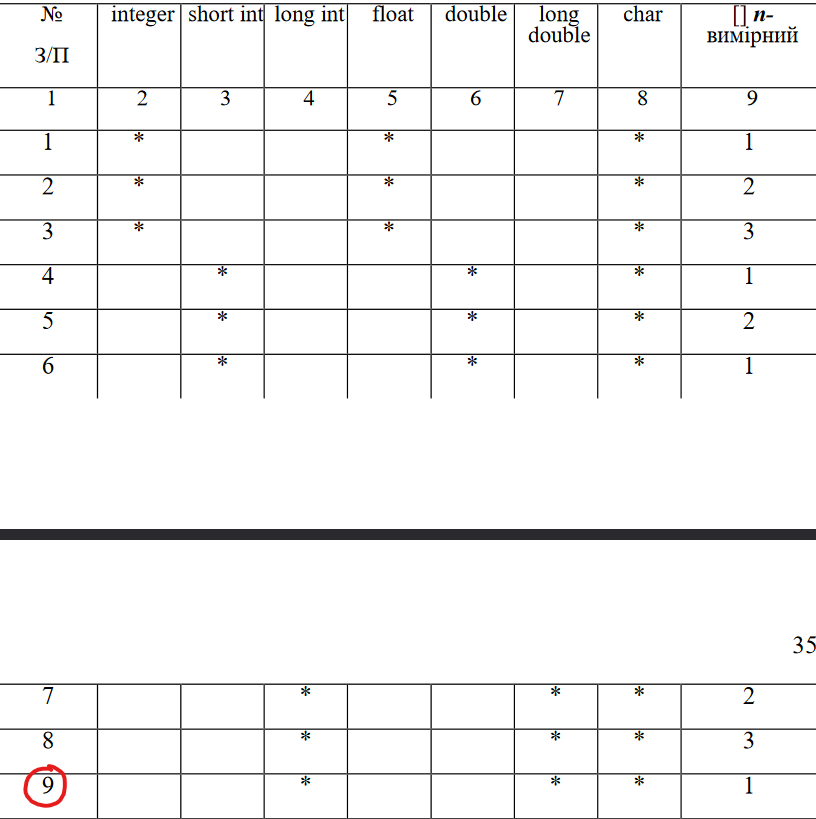
\includegraphics[width=16cm]{reports/algos/lab3/assets/1.png}
\end{figure}

\clearpage
\textbf{Реалізація програми:}

\begin{lstlisting}[style=customc]
#include <math.h>
#include <stdio.h>
#include <stdlib.h>
#include <time.h>

#include "general_utils.h"

void printBinary(unsigned char byte) {
    for (int i = 7; i >= 0; i--) {
        int bit = (byte >> i) & 1;
        printf("%d", bit);
    }
    printf(" ");
}

void printInternalLongInt(long int val){
    printf("\033[35mMachine code of (long int = %ld)\033[0m: ", val);
    for (size_t i = 0; i < sizeof(long int); i++)
    {
        printBinary((unsigned char)(val >> (i * 8)));
    }
    printf("\n");
}

void printInternalLongDouble(long double val){
    printf("\033[35mMachine code of (long double = %Lf)\033[0m: ", val);
    unsigned char *longDoubleBytes = (unsigned char*)&val;
    for (int i = 0; i < sizeof(long double); i++) {
        printBinary(longDoubleBytes[i]); 
    }
    printf("\n");
}

void printInternalChar(char val) {
    printf("\033[35mMachine code of (char = '%c')\033[0m: ", val);
    printBinary((unsigned char)val);
    printf("\n");
}

void printInternalInt(int val) {
    printf("\033[35mMachine code of (int = %d)\033[0m: ", val);
    for (size_t i = 0; i < sizeof(int); i++) {
        printBinary((unsigned char)(val >> (i * 8)));
    }
    printf("\n");
}

void printInternalIntArray(int* arr, size_t size) {
    printf("\033[34mMachine code of array with int values\033[0m:\n\n");
    for (size_t i = 0; i < size; i++) {
        printf("Елемент %zu: ", i);
        printInternalInt(arr[i]);
    }
}

void task1() {
    long int longIntValue = 78L;            
    long double longDoubleValue = 3.14159L;  
    char charValue = 'A';  

    int arr[5] = {1, 2, 3, 4, 5};

    highlightText("Machine code of values:", "blue");
    printf("\n");                  

    printInternalLongInt(longIntValue);
    printInternalLongDouble(longDoubleValue);
    printInternalChar(charValue);
    printf("\n");
    printInternalIntArray(arr, 5);
}
\end{lstlisting}

2) Для відображення всіх 8 бітів у байті було створено функцію \textbf{printBinary}, вона робить це шляхом бінарного здвигу вправо на кількість позицій на поточній ітерації та застосовує маску \textbf{"И" з одиницею} щоб отримати тільки останній біт та вивести його.
     Все це вона робить з типом \textbf{unsigned char}, бо він зручний для відображення одного байту.

\begin{lstlisting}[style=customc]
void printBinary(unsigned char byte) {
    for (int i = 7; i >= 0; i--) {
        int bit = (byte >> i) & 1;
        printf("%d", bit);
    }
    printf(" ");
}
\end{lstlisting}

3) Вивід \textbf{long int} здійснюється за допомогою функції \textbf{printInternalLongInt}, вона прийме в себе значення та виведе його машинне представлення у такій кількості байт який займає тип данних \textbf{long int}:

\begin{lstlisting}[style=customc]
void printInternalLongInt(long int val){
    printf("\033[35mMachine code of (long int = %ld)\033[0m: ", val);
    for (size_t i = 0; i < sizeof(long int); i++)
    {
        printBinary((unsigned char)(val >> (i * 8)));
    }
    printf("\n");
}
\end{lstlisting}

4) Вивід \textbf{long double} здійснюється за допомогою функції \textbf{printInternalLongDouble}, вона прийме в себе значення та виведе його машинне представлення у такій кількості байт який займає тип данних \textbf{long double}:

\begin{lstlisting}[style=customc]
void printInternalLongDouble(long double val){
    printf("\033[35mMachine code of (long double = %Lf)\033[0m: ", val);
    unsigned char *longDoubleBytes = (unsigned char*)&val;
    for (int i = 0; i < sizeof(long double); i++) {
        printBinary(longDoubleBytes[i]); 
    }
    printf("\n");
}
\end{lstlisting}

\clearpage
5) Вивід \textbf{char} здійснюється за допомогою функції \textbf{printInternalChar}, вона прийме в себе значення та виведе його машинне представлення у такій кількості байт який займає тип данних \textbf{char}:

\begin{lstlisting}[style=customc]
void printInternalChar(char val) {
    printf("\033[35mMachine code of (char = '%c')\033[0m: ", val);
    printBinary((unsigned char)val);
    printf("\n");
}
\end{lstlisting}


6) Виведення масиву (в моєму випадку масиву цілих чисел) відбувається за допомогою почергового представленя у машиному вигляді кожного елементу масиву, для цього була додана функція \textbf{printInternalInt} для виводу машиного представлення цілих чисел:

\begin{lstlisting}[style=customc]
void printInternalInt(int val) {
    printf("\033[35mMachine code of (int = %d)\033[0m: ", val);
    for (size_t i = 0; i < sizeof(int); i++) {
        printBinary((unsigned char)(val >> (i * 8)));
    }
    printf("\n");
}

void printInternalIntArray(int* arr, size_t size) {
    printf("\033[34mMachine code of array with int values\033[0m:\n\n");
    for (size_t i = 0; i < size; i++) {
        printf("Елемент %zu: ", i);
        printInternalInt(arr[i]);
    }
}
\end{lstlisting}

7) Результати роботи програми:
\begin{figure}[h!]
    \centering
    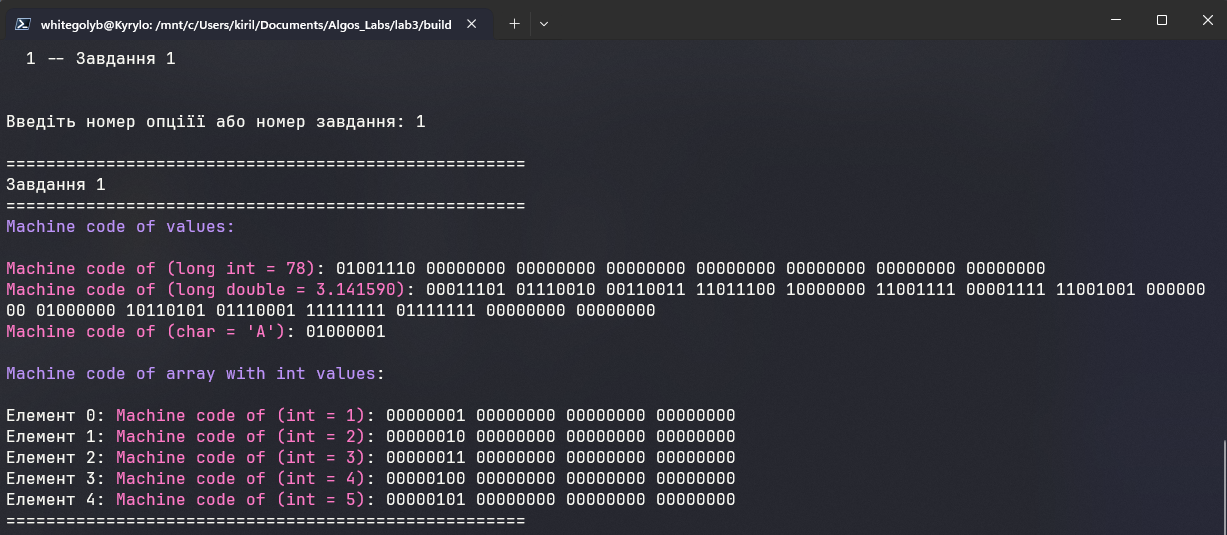
\includegraphics[width=16cm]{reports/algos/lab3/assets/2.png}
\end{figure}

\clearpage
Можна зазначити що від`ємні числа показаються у додатковому коді, наприклад змінимо елементи масиву, це можна легко перевірити якщо власноруч порахувати:
\begin{figure}[h!]
    \centering
    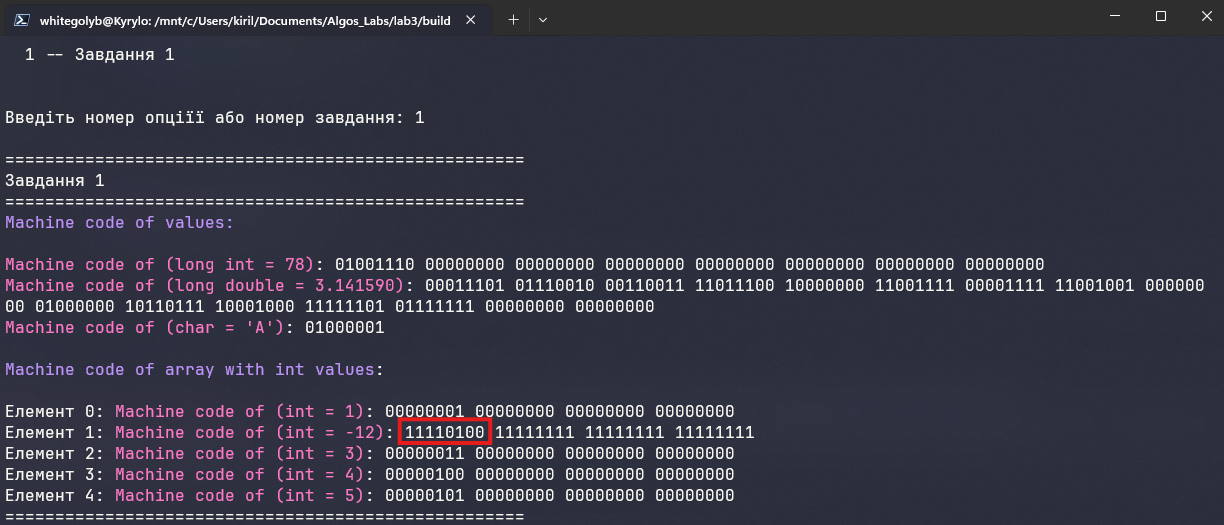
\includegraphics[width=16cm]{reports/algos/lab3/assets/3.png}
    \caption{Представленя у додатковому коді числа -12 у програмі}
\end{figure}

\begin{figure}[h!]
    \centering
    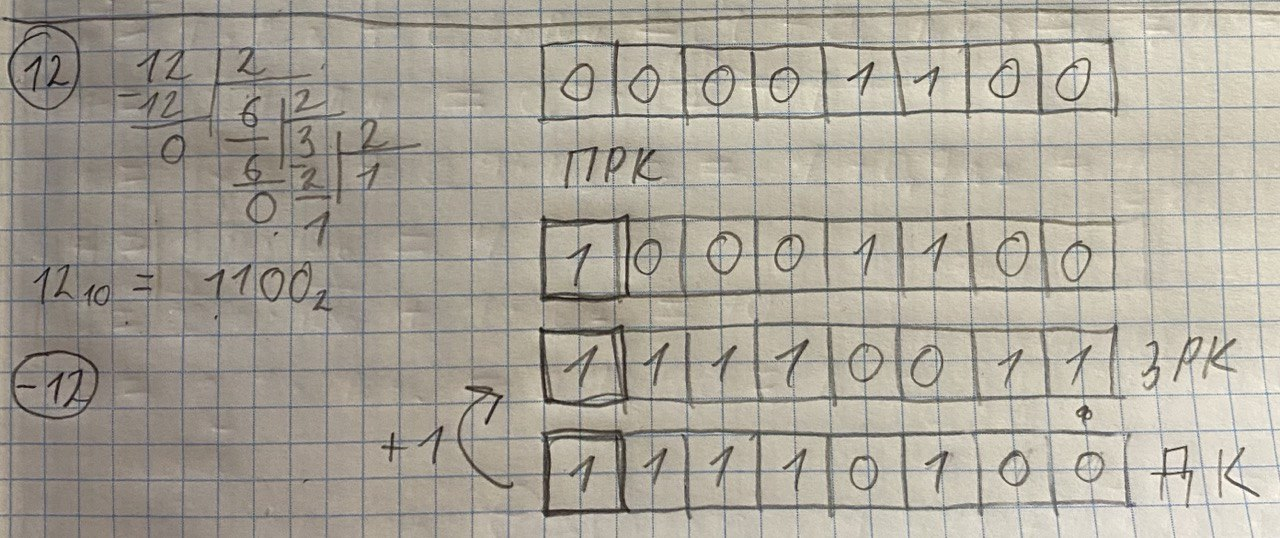
\includegraphics[width=16cm]{reports/algos/lab3/assets/4.jpg}
    \caption{Представленя у додатковому коді числа -12 власноруч}
\end{figure}

\clearpage
\section{Висновки}

